\begin{figure}[h!]
   \centering
   \begin{subfigure}[b]{0.4\textwidth}
      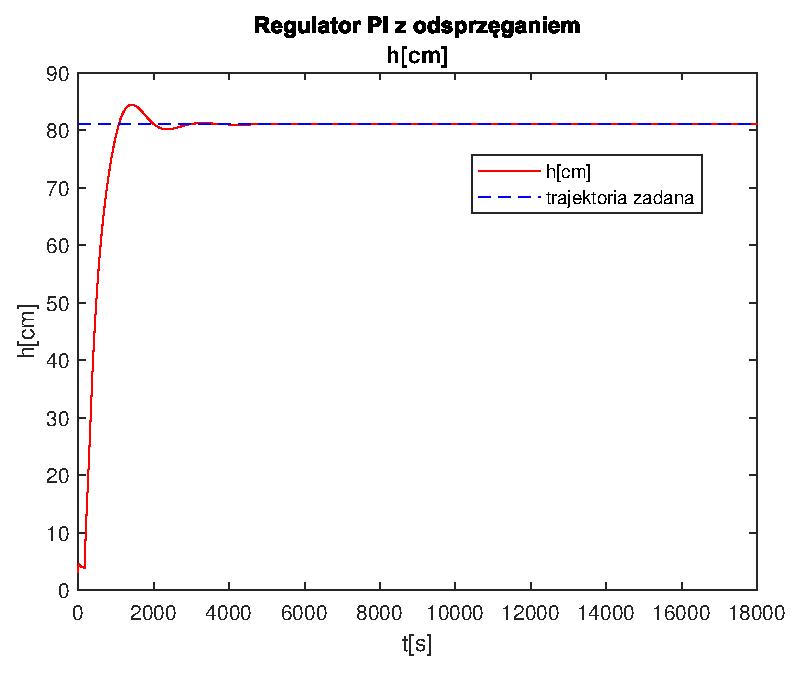
\includegraphics[width=1\linewidth]{img/PI/decoupler/noDisturbance/PIDecouplerH0.eps}
      \caption{}
      \label{fig:fig:PIDecoupler01}
   \end{subfigure}
       
   \begin{subfigure}[b]{0.4\textwidth}
      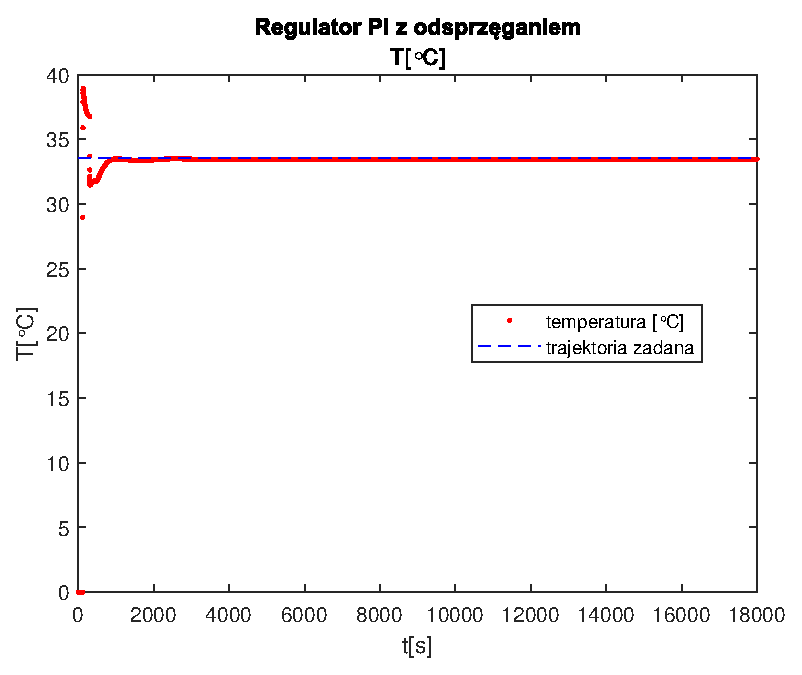
\includegraphics[width=1\linewidth]{img/PI/decoupler/noDisturbance/PIDecouplerT0.eps}
      \caption{}
      \label{fig:fig:PIDecoupler02}
   \end{subfigure}
       
   \begin{subfigure}[b]{0.4\textwidth}
      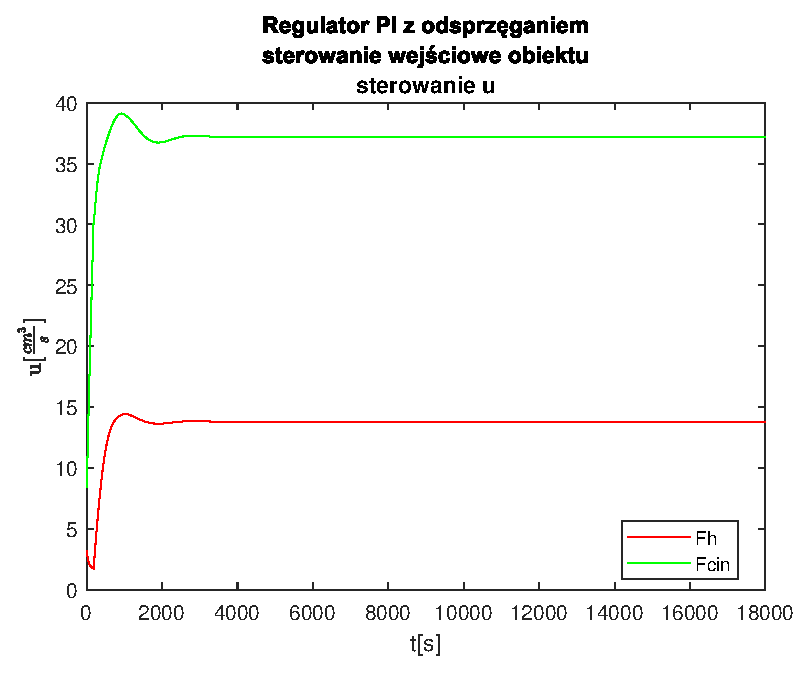
\includegraphics[width=1\linewidth]{img/PI/decoupler/noDisturbance/PIDecouplerControl0.eps}
      \caption{}
      \label{fig:fig:PIDecoupler03}
   \end{subfigure}
       
   \begin{subfigure}[b]{0.4\textwidth}
      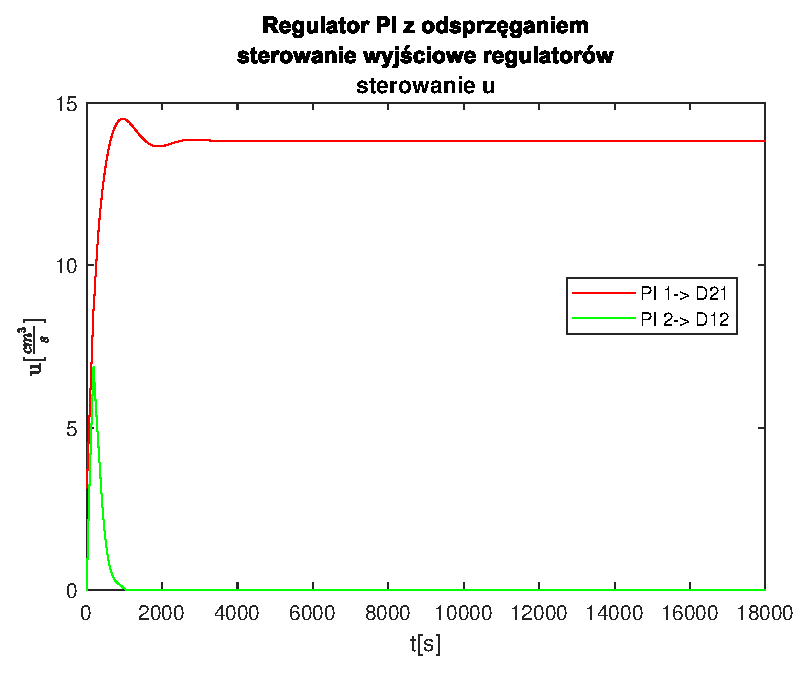
\includegraphics[width=1\linewidth]{img/PI/decoupler/noDisturbance/PIDecouplerControlD0.eps}
      \caption{}
      \label{fig:fig:PIDecoupler04}
   \end{subfigure}
       
   \caption{Wykresy dla regulatora PI z odsprzeganiem.}
   \label{fig:PIDecoupler0}
\end{figure}
           
